\documentclass{article}
\usepackage{tikz}
\usetikzlibrary{external}
\tikzexternalize[mode=list and make]

\tikzset{
    % Defines a custom style which generates BOTH, .pdf and .png export
    % but prefers the .png on inclusion.
    %
    % This style is not pre-defined, you may need to copy-paste and
    % adjust it.
    png export/.style={
        external/system call/.add={}{; convert -density 300 -transparent white "\image.pdf" "\image.png"},
        %
        /pgf/images/external info,
        /pgf/images/include external/.code={%
            \includegraphics
            [width=\pgfexternalwidth,height=\pgfexternalheight]
            {##1.png}%
        },
    },
    %
    png export,% ACTIVATE
}

\begin{document}

{
% Here we specify the figure will be converted and inserted as PNG
\tikzset{png export}
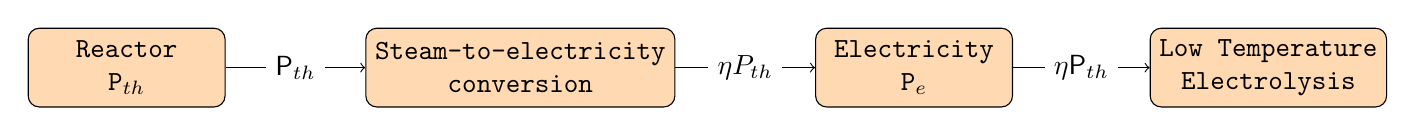
\begin{tikzpicture}[
    base/.style = {rectangle, rounded corners, draw=black,
minimum width=3cm, minimum height=1cm,
text centered, font=\sffamily},
process/.style = {base, minimum width=2.5cm, fill=orange!30,
font=\ttfamily},
node distance=3cm,
every node/.style={fill=white, font=\sffamily}, align=center
]

  \node (reactor) [process] {Reactor\\P$_{th}$};
  \node (steam1)  [process, right of=reactor, xshift=2.cm] {Steam-to-electricity\\conversion};

  \node (elect)   [process, right of=steam1, xshift=2.cm] {Electricity\\P$_e$};
  \node (hte)   [process, right of=elect, xshift=1.5cm] {Low Temperature\\Electrolysis};

 \draw[->]      (reactor) -- (steam1) node[midway] {P$_{th}$};
 \draw[->]      (steam1) -- (elect) node[midway] {$\eta P_{th}$};
 \draw[->]      (elect) -- (hte) node[midway] {$\eta$P$_{th}$};

\end{tikzpicture}
}

\end{document}

% To compile do make; make -f hte1.makefile


